% !TeX root = ../main.tex
\section{Results}
\label{sec:model_comparison}
%
The discretised-reflection model now allows us to revisit and extend established results on semiconductor lasers with FBG feedback.
We first show that the EGM structure predicted by the model reproduces earlier findings from the literature with excellent agreement, while providing a more complete classification through analytic expressions and continuation methods.
Building on this foundation, we then examine laser stability, demonstrating how reflection zeros interact with the laser centre frequency and relaxation oscillations in close parallel to previous studies, but on a far more concrete basis enabled by the present formulation.
%
%
\subsection{EGM Structure}
\label{subsec:EGM_structure}
%
\subsubsection{Comparison to multiple reflection FBG feedback}
\label{subsubsec:naumenko}
%
A considerably more elaborate treatment of FBG feedback was developed by Naumenko \textit{et al.} \cite{naumenko2003characteristics,naumenko2004slow}, who modeled the feedback term $F(t)$ as the inverse Fourier transform of the product of the delayed electric field spectrum and the grating reflection spectrum $\rho(\w)$, see Appendix~\ref{app:EC_multiple}.
This formulation, summarised in the introduction, enabled them to capture the essential role of spectral filtering in reorganising EGMs by means of a Green-function formalism.
Their model further incorporated nonlinear gain compression and thermally induced frequency chirp, which strongly affect stability under current modulation.
When these additional effects are neglected, and appropriate simplifications are made, their system reduces to the discretised-reflection formulation derived here (Appendix~\ref{app:EC_multiple}), with parameter set $(\a, P, T, \tau, C_p) = (4, 0.5, 123, 512, 0)$ and varying grating parameters $\eta$, $\wB$, and $\wz$.
%
\par
%
In their analysis, EGMs were constructed through a Green-function expansion rather than closed-form analytical conditions, leading to an involved but tractable calculation of mode frequencies.
As noted earlier, Naumenko \textit{et al.} identified the appearance of “satellite” EGM branches, separated from the central EGM ellipse by the reflection zeros of the FBG, as the bandwidth $\wz$ narrowed or detuning $\wB$ increased.
This insight was critical in establishing the connection between spectral features of the grating and the global organisation of EGMs, but the complexity of their feedback term limited the use of continuation methods and left the bifurcation structure only partially characterised.
%
\begin{figure}[!t]
    \centering

        \begin{overpic}[width=0.74\linewidth]{Images/rB_003_annotated.pdf}
            \put(-2,44){(b)}
            \put(-2,96){(a)}
        \end{overpic}\\
        \hspace{-2.2em}
        \begin{overpic}[width=0.65\linewidth]{Images/Naumenko_EGM_rB003.pdf}
            \put(-5,80){(c)}
        \end{overpic}

    \caption{Comparison of EGM structures from the multiple-reflection model of Naumenko \textit{et al.} and the discretised-reflection model.
    Panel (a) shows the common FBG frequency responses corresponding to bandwidths with reflection zeros at $1/3$, $4/3$, and $20/3\,$GHz, giving nondimensionalised locations $\wz = 0.016\pi, \; 0.064\pi, \; 0.32\pi$.
    A constant reflectivity $R=\sqrt{0.001}$ yields an effective feedback rate $\eta=0.085$.
    Panels (b) and (c) plot the resulting EGMs for these bandwidths using the multiple-reflection formulation and the discretised model, respectively.
    In both cases, EGM branches are distinguished by circles, diamonds, and squares, while the MGM is marked by $\times$.}
    
    \label{fig:Naumenko_rB003}
\end{figure}
%
\begin{figure}[!t]
    \centering

        \begin{overpic}[width=0.725\linewidth]{Images/rB_02_annotated.pdf}
            \put(-2,45){(b)}
            \put(-2,96){(a)}
        \end{overpic}\\
        \hspace{-0.3em}
        \begin{overpic}[width=0.612\linewidth]{Images/Naumenko_EGM_rB02.pdf}
            \put(-12,87){(c)}
        \end{overpic}

    \caption{Comparison of EGM structures for a detuned FBG under moderate feedback shown in (a) from the multiple-reflection model (b) and the discretised-reflection model (c) .
    Here, a reflectivity $R=\sqrt{0.05}$ gives an effective feedback rate $\eta=0.600$, the first reflection zero at $10/3\,$GHz corresponds to $\wz=0.16\pi$, and a detuning of $8\,$GHz yields $\wB=0.384\pi$.}

    \label{fig:Naumenko_rB02}
\end{figure}
%
\par
%
Figure~\ref{fig:Naumenko_rB003} compares the EGM structures obtained from the multiple-reflection model of Naumenko \textit{et al.} \cite{naumenko2003characteristics} with those predicted by the discretised-reflection formulation for varying grating bandwidth.
For the parameter set under consideration, the layer number $N=10$ was chosen, which exceeds the minimal value $N_\text{min}=7$ required for validity according to \eqref{eq:Nmin}.
The solutions are plotted in the frequency–intensity plane ($I=|E|^2$), rather than the more common $(\w_s,N_s)$-projection, which results in an inversion of the cavity-mode structure about the frequency axis.
Conversion of bandwidths from hertz to the nondimensionalised form $\wz$ was performed using the quoted photon lifetime $\tau_p=24$ ps \cite{naumenko2003characteristics}.
%
\par
%
In the case of zero detuning and weak feedback (Figure~\ref{fig:Naumenko_rB003}), excellent agreement is achieved between the two models.
For a wide Bragg-reflector bandwidth (here a main-lobe width of $40/3\,$GHz, corresponding to $2\wz=0.64\pi$ in nondimensional form), the EGMs trace a closed curve strongly resembling the ECM ellipse of the COF case.
The maximal gain mode (MGM), marked by $\times$, is located near the edge of the left-hand side of this curve.
Further information is provided in the discretised case, as the closed curve which traces the EGM solutions given by \eqref{eq:discretised_Ns_curve} is also shown in (c), giving a clearer picture of the seperate components.
As the FBG bandwidth narrows, the number of EGMs decreases and the EGM curve contracts, remaining confined within the main lobe of the reflection spectrum.
This behaviour is fully consistent with the analytic results of Section~\ref{subsec:EGM_discretised} and with earlier studies of Lorentzian-filter feedback \cite{yousefi1999dynamical}.
%
\par
%
For sufficiently narrow bandwidths, additional satellite EGMs appear, marked with triangles in Figure~\ref{fig:Naumenko_rB003}.
These satellites arise from the side lobes of the FBG reflection spectrum and are a distinctive feature of grating-based feedback.
Notably, they do not appear in the single Lorentzian-filter model under zero detuning, underscoring the richer spectral structure captured here.
In this regime, the MGM shifts closer to the Bragg frequency, as expected from physical considerations.
%
\par
%
When the feedback strength is increased and the grating is detuned from the free-running laser frequency (Figure~\ref{fig:Naumenko_rB02}), the EGM branches themselves become detuned and reorganise into three disjoint curves.
These correspond to the main reflection lobe and the two nearest side lobes.
An analogous splitting was observed in the Lorentzian-filter model \cite{yousefi1999dynamical}, but only up to two branches could form \cite{green2006mode}.
The present results therefore highlight the additional richness of the FBG spectrum, where multiple side lobes can sustain distinct EGM families.
%
\par
%
Across all regimes, the discretised-reflection model reproduces the locations of EGM components, the MGM, and the number of EGM solutions with excellent accuracy compared to the multiple-reflection formulation.
The main discrepancy lies in distortions along the intensity axis, most visible under strong feedback, which can be attributed to the absence of gain-suppression effects in the simplified discretised model.
Nevertheless, the structural agreement between the two approaches confirms that the discretised-reflection formulation successfully captures the essential organisation of mode solutions under FBG feedback.
This agreement gives further validation for this model as a tractable framework for extended spectral and stability analysis.
%
\subsubsection{Bifurcations of EGMs}
\label{subsubsec:EGM_folds}
%
\begin{figure}[t]
    \centering

    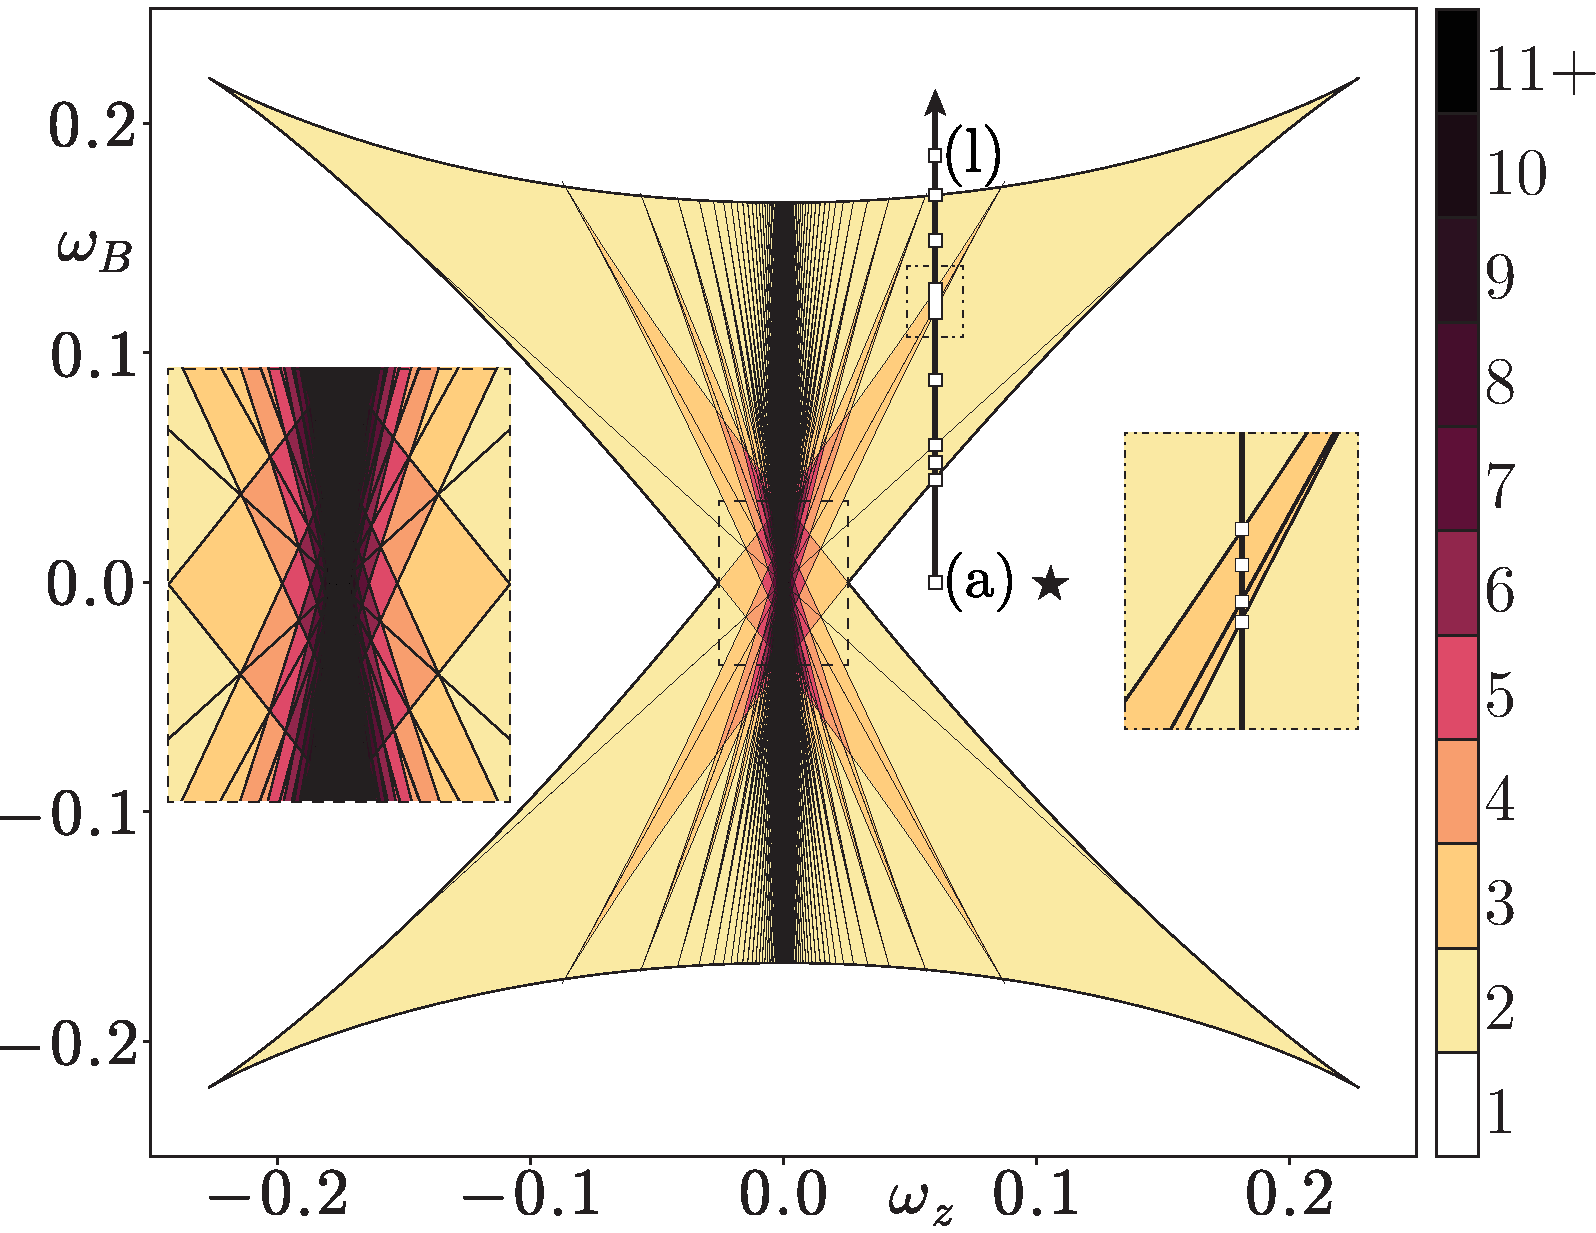
\includegraphics[width=\linewidth]{Images/EGM_components_2D_coloured_with_closeup.pdf}

    \caption{Regions of the $(\wz, \wB)$-plane showing the number of isolated EGM components, with values up to 11 indicated by the colourbar.
    The inset provides a close-up of the region with the highest component density.
    Squares along the line $\wz=0.06$ mark the parameter values used in Figure~\ref{fig:EGM_fold_varywB} while the black star corresponds to the single EGM component observed in Figure~\ref{fig:discretised_EGM_varyN}(b)-(d).
}

    \label{fig:EGM_components}
\end{figure}
%
\begin{figure}[!t]
    \centering
    \begin{overpic}[width=\linewidth]{Images/EGM_fold_varywB_wz006.pdf}
        % Row a
        \put(11.5,95.9){(a)}
        \put(36.3,95.9){(e)}
        \put(61.2,95.9){(i)}
        % Row b
        \put(11.5,72.1){(b)}
        \put(36.3,72.1){(f)}
        \put(61.2,72.1){(j)}
        % Row c
        \put(11.5,48.5){(c)}
        \put(36.3,48.5){(g)}
        \put(61.2,48.5){(k)}
        % Row d
        \put(11.5,24.6){(d)}
        \put(36.3,24.6){(h)}
        \put(61.2,24.6){(l)}
    \end{overpic}

    \caption{Graph of the EGM component function $G(\w_s)$ from \eqref{eq:EGM_components} for $\wz = 0.06$ and varying $\wB$, whose particular values are indicated by dots along the line $\wz=0.06$ in Figure~\ref{fig:EGM_components}.
    The roots (hollow circles) bound intervals of $\w_s$ values corresponding to EGM components (thick lines); one interval always contains $\w_s = 0$ (the free running laser mode) and another contains the grating's Bragg frequency for $\wB \in [0.04505, 0.16895]$.
    }

    \label{fig:EGM_fold_varywB}
\end{figure}
%
\begin{figure*}[!t]
    \flushleft
    \hspace{1em}
    \begin{overpic}[width=0.93\linewidth]{Images/EGM_components_varyN.pdf}
        % Row a
        \put(3.6, 59.8){(a)}
        \put(36, 59.8){(b)}
        \put(68.5, 59.8){(c)}
        % Row b
        \put(3.6, 30.5){(d)}
        \put(36, 30.5){(e)}
        \put(68.5, 30.5){(f)}
    \end{overpic}

    \caption{Fold bifurcations of EGM components in the $(\wz,\wB)$-plane for varying layer number $N \in [5, 10, 20, 50, 100, 1000]$ in panels (a)-(f), respectively.
    Invalid regions where $N < N_\text{min}$ according to case 1 of \eqref{eq:Nmin} are shaded in grey, while invalid regions according to case 2 are shaded in red.}

    \label{fig:EGM_components_varyN}
\end{figure*}
%
Having validated the model against prior modelling approaches, we now turn to one of its central advantages: the ability to analyse global EGM bifurcation structure directly and analytically.
In particular, the discretised equations yield closed-form conditions for the creation and annihilation of EGM components, providing global insight into how the mode organisation depends on detuning, bandwidth, and reflectivity.
%
\par
%
The number of EGM components can be determined by equating the EGM envelope $f_\text{env}(\w_s)$ in \eqref{eq:discretised_ws_envelope} with $g(\w_s)$, which amounts to seeking the roots of
%
\begin{equation}
    \label{eq:EGM_components}
    G(\w_s) = \w_s^2 - (1+\a^2)\left( \eta \, (1-t) \frac{S_N}{S} \right)^2.
 \end{equation}
%
The real roots of $G(\w_s)$ mark the intersections of the envelope with $g(\w_s)$ and thus bound the intervals of $\w_s$ corresponding to distinct EGM components.
In this way, $G(\w_s)$ serves as a compact geometric picture of the global mode structure.
Changes in the number of EGM components occur when fold points of the envelope become tangent to $g(\w_s)$.
Such fold bifurcations arise when the derivative of $G(\w_s)$ with respect to $\w_s$ vanishes, giving the condition
%
\begin{gather}
    \label{eq:EGM_components_fold}
    \begin{aligned}
        \frac{\partial G}{\partial \w_s} &= \dt (1+\a^2)\left( \eta \, (1-t) \frac{S_N}{S} \right)^2 \times \\ 
        &\bigg(  \frac{t}{S^2} \sin(\phi_\text{F}) - N \frac{t^{N}}{{S_N}^2}\sin(N\phi_\text{F}) \bigg) + \w_s = 0.
    \end{aligned}
\end{gather}
%
\par
%
Having established these conditions, we now turn to a global view of how the number of EGM components evolves across the $(\wz,\wB)$-plane.
The loci of fold bifurcations can be tracked using the pseudo-arclength continuation routines of \texttt{DDE-BifTool} \cite{sieber2014dde}, which solve the coupled conditions $G(\w_s)=0$ and $\sfrac{dG(\w_s)}{d\w_s}=0$ simultaneously.
The resulting continuation curves, shown in Figure~\ref{fig:EGM_components} for $N=1000$, partition the $(\wz,\wB)$-plane into regions with different numbers of isolated EGM components.
In the white region only a single component exists, while inside the shaded region two or more components are present.
The bounding fold curves meet at cusp points, marking the transition between single- and multi-component regimes.
%
\par
%
Strikingly, the boundary between one and two components exhibits the same cusp-shaped structure as the corresponding bifurcation diagram for FOF feedback (cf. \cite{green2006mode}, Figure~3(a)), albeit using different parameter values.
Within the multi-component region, additional fold bifurcations arise as $\wz$ and $\wB$ vary, leading to the emergence of further EGM components.
These new components appear through two-to-three component transitions, organised by families of fold curves that accumulate and terminate at cusp points along the upper and lower edges of the primary one-to-two boundary.
As these fold curves overlap, regions with more than three components are created, as illustrated in the inset of Figure~\ref{fig:EGM_components}, revealing how increasingly intricate mode structures emerge in a systematic fashion.
Finally, the entire bifurcation structure scales linearly with the effective feedback strength $\eta (1-t)\sqrt{1+\alpha^2}$: the cusp-shaped regions preserve their geometry but expand proportionally with feedback.
%
\par
%
To illustrate in detail the behaviour summarised in Figure~\ref{fig:EGM_components}, transitions in the number of EGM components is shown in Figure~\ref{fig:EGM_fold_varywB}(a)--(l).
Here, the function $G(\w_s)$ is plotted for fixed $\wz=0.06$ and increasing detuning $\wB \in [0,0.175]$.
Dashed and dotted vertical lines mark the free-running laser frequency $\w_s=0$ and the Bragg frequency $\w_s=\wB$, respectively.
At $\wB=0$ (panel (a)), a single wide EGM component exists, containing both $\w_s=0$ and $\w_s=\wB$.
The number of components changes whenever a fold of the envelope passes through $G(\w_s)=0$: for example, in panel (b) a transition from one to two components occurs, corresponding exactly to the outer boundary of Figure~\ref{fig:EGM_components}.
We remark that that initially both $\w_s=0$ and $\w_s=\wB$ remain in the same component as shown in panel (c).
%
\par
%
Fold curves nested inside the cusp-shaped region, also visible in Figure~\ref{fig:EGM_components}, correspond to solutions of $G(0)=0$, that is, they occur precisely at the laser frequency.
Crossing such a curve does not change the total number of components; instead, it marks the condition where a reflection zero of the FBG spectrum coincides with the laser frequency, yielding the simple parametrisation $\wB = n\wz, \; n \in \mathbb{Z}$.
Panel (d) illustrates this case: beyond it, the laser frequency and Bragg frequency reside in different components.
As detuning increases, a second envelope fold crosses $G(\w_s)=0$ (panel (f)), marking entry into the region associated with the second cusp along the line $\wz = 0.06$.
This is followed by another fold through $\w_s=0$ (panel (g)), after which an additional “mixed” component appears containing neither $\w_s=0$ nor $\w_s=\wB$.
Such mixed-frequency components are a distinctive feature of FBG feedback and have no analogue in the FOF case, where at most two components exist, one containing $\w_s=0$ and the other $\w_s=\wB$ \cite{green2006mode}.
With further detuning, the mixed component is annihilated first, followed by the Bragg-frequency component, as shown in panels (i)--(l).
Ultimately, only a single EGM component containing the laser’s free-running frequency remains.
An animation of the evolution of EGM components in the $(\w_s, N_s)$-plane as $\wB$ varies is provided in the supplementary material (\texttt{EGM\_wB\_animation.gif} [500KB]) while an explicit one-component EGM structure shown in Figure~\ref{fig:EGM_components_varyN}(c) is indicated by the black star in \ref{fig:EGM_components}.
%
\par
%
To conclude, Figure~\ref{fig:EGM_components_varyN} presents the bifurcation diagram of Figure~\ref{fig:EGM_components} for varying layer numbers $N$, illustrating how insufficient $N$ introduces non-physical EGM components that distort the bifurcation structure.
The outer one-to-two component boundary remains largely unaffected by $N$, but the inner fold curves are highly sensitive: as $N$ decreases, the two-to-three fold curves that meet at cusp points extend well beyond the upper and lower boundaries.
To make these distortions explicit, the invalid regions predicted by \eqref{eq:Nmin} are overlaid.
The first case, shaded grey, corresponds to the onset of unphysical side lobes whose amplitudes increase due to repetition of the reflection spectrum, as illustrated in column (1) of Figure~\ref{fig:discretised_EGM_minimumN}.
The second case, shaded red, marks the appearance of repeated main lobes of the reflection spectrum, as shown in column (2) of Figure~\ref{fig:discretised_EGM_minimumN}.
Together, these two conditions account for all invalid regions, apart from a small number of fold curves that extend slightly beyond the upper and lower one-to-two component boundaries.
%
\par
%
In summary, the proposed model not only reproduces the EGM structures obtained in earlier multiple-reflection analyses, but also extends them through explicit bifurcation diagrams and continuation.
This yields, for the first time, a complete and analytically grounded classification of how EGM components emerge, interact, and disappear across parameter space.
With this rigorous spectral foundation established, we now turn to the dynamical stability of these modes.
In the next section, we revisit previous stability results under FBG feedback, but now place them on a firmer basis by exploiting advanced continuation techniques to deliver a more precise and comprehensive characterisation of the system’s behaviour.
%
%
\subsection{Stability Fluctuations}
\label{subsec:lichaos_skenderas}
%
\begin{figure}[t]
    \centering
    \begin{overpic}[width=0.9\linewidth]{Images/Reflection_zero_overlap.pdf}
        \put(2,86){(a)}
        \put(2,43){(b)}
    \end{overpic}
    \caption{Schematic illustrating how the reflection zeros of the FBG spectrum align with intrinsic laser frequencies.
    (a) Overlap with the free-running frequency $\w_s=0$ suppresses the central lasing mode.
    (b) Overlap with the relaxation oscillation (RO) frequency $\w_\text{RO}$ suppresses the characteristic sidebands, stabilising the output.}
    \label{fig:zero_overlap}
\end{figure}
%
Having established the global organisation of EGMs in terms of detuning and bandwidth, we now turn to their stability.
Although a given parameter set may permit one or more EGM components, the actual output of the laser is determined by the stability of its modes.
In the context of FBG feedback, physically, stability is in part influenced by how reflection zeros of the FBG spectrum align with characteristic frequencies of the solitary laser, as illustrated in Figure~\ref{fig:zero_overlap}.
%
\par
%
The first stabilisation case concerns the free-running laser frequency at $\w_s=0$.
If a reflection zero coincides with this frequency, the central lasing frequency is suppressed, removing a potential instability through which fluctuations from the steady-state would otherwise grow.
This behaviour is illustrated in Figure~\ref{fig:zero_overlap}(a) where a spectrum is detuned from $\wB=0$ (black) to $\wB = \wz$ (grey) and $\wB = 2\wz$ (light grey), causing the laser's free-running frequency to align with the spectrum's first and second zeros, respectively.
%
\par
%
The second stabilisation case involves the relaxation oscillation (RO) frequency $\w_\text{RO}=\sqrt{2P/T}$, which arises from the coupled dynamics of photon and carrier densities: when the carrier population is perturbed, it overshoots its steady state, producing damped oscillations in output intensity at $\w_\text{RO}$ that appear as symmetric sidebands in the spectrum.
Aligning a reflection zero with $\w_\text{RO}$ damps these sidebands and suppresses RO-driven instabilities, thereby stabilising the laser output.
Figure~\ref{fig:zero_overlap}(b) illustrates this behaviour by decreasing the bandwidth of a spectrum with $\wz>\w_\text{RO}$ (black) until $\wz = \w_\text{RO}$ (grey) and $\wz = \w_\text{RO} / 2$ (light grey), causing the laser's RO frequencies to again align with the spectrum's first and second zeros, respectively.
%
\par
%
In what follows, we analyse these two stabilisation mechanisms in detail by comparing two-parameter bifurcation diagrams obtained with convolution-based formulations of FBG feedback \cite{li2015chaotic,skenderas2024impact} against those from the discretised-reflection model.
This serves both to validate the proposed model’s ability to reproduce known stability features and to demonstrate how more advanced mathematical techniques extend the analysis, yielding a deeper understanding of the destabilisation mechanisms present under FBG feedback.
We begin with the case of alignment at the laser free-running frequency, before turning to alignment at the laser RO sidebands.
%
%
\subsubsection{Interaction between FBG zeros at the laser frequency}
\label{subsubsec:lichaos}
%
Figure~\ref{fig:lichaos} compares two-parameter dynamical mappings of the laser output under FBG feedback, obtained using both the convolution formulation \cite{li2012distributed,li2015chaotic,li2020stable} and the discretised-reflection formulation.
The parameter set is $(\a, P, T, \tau) = (-3.2, 0.61, 93, 252)$, with a grating bandwidth of $f_l = 5$ GHz corresponding to a reflection-zero spacing $\wz = 0.058612$, while the negative value of $\alpha$ reflects the sign convention adopted in the convolution-based model.
Equivalent parameter values were determined by a sequence of approximations and nondimensionalisations of the convolution formulation; full details are provided in Appendix~\ref{app:Li_chaos_nondim}.
Given that increasing the feedback rate tends to destabalise the laser's output, the frequency selective stabilisation mechanism under consideration can be analysed through the correlation between the feedback strength required to destabalise the laser and the FBG reflectivity spectrum.
Consequently, the parameters $\eta$ and $\wB$ are varied to explore the resulting stability fluctuations.
Over the range of interest, $\eta_\text{max} = 0.24$ and $|\wB|_\text{max} = 8 \times 0.058612$, so the layer number was set to $N=30$, safely exceeding the minimum requirement $N_\text{min}=22$ given by \eqref{eq:Nmin}.
%
\par
%
Both FBG feedback formulations describe the dynamics in the parameter plane of feedback strength ($\xi_f$ in the convolution model and equivalent $\eta$ here) and detuning $\Delta f$.
In the convolution case, reproduced from \cite{li2015chaotic} Fig.~3 [panel (a)], the output is classified as steady state (white), period-one oscillatory (red), period-two oscillatory (yellow), quasi-periodic (gray), and chaotic (black).
The discretised-reflection model [panels (b,c)] reproduces these regimes in close agreement: classified through periodicity as steady state (white), period-one (red), period-two (yellow), and higher-period represented by grey and black.
For the discretised model, periodicity was classified by integrating \eqref{eq:LK_discretised} using the 3-step  Adams-Bashforth-Moulton predictor-corrector method with a time step $\Delta t = 0.5$ up to $t = 5\e5$ and counting local maxima of the intensity $I = |E|^2$ in the final 10\% of the transient.
To expose the underlying bifurcation structure, panel (b) overlays Hopf bifurcations of the steady EGM branches (red curves) computed with \texttt{DDE-BifTool}, while panel (c) overlays the Kaplan-Yorke dimension of any detected chaotic attractor (coloured by the accompanying scale), computed from the full Lyapunov exponent spectrum.
%
\par
%
\begin{figure}[!t]
    \flushleft
    \hspace*{0.8em}
    \begin{overpic}[width=0.825\linewidth]{Images/Li_chaos_heatmap_image.pdf}
        \put(-2,77){(a)}
    \end{overpic}\\
    \vspace{-0.5em}
    \hspace*{1em}
    \begin{overpic}[width=0.97\linewidth]{Images/discretised_Lichoatic_wBeta_comparison_hopfs_minbifs_ai.pdf}
        \put(-2,65){(b)}
    \end{overpic}\\
    \vspace{-0.5em}
    \hspace*{1em}
    \begin{overpic}[width=0.975\linewidth]{Images/discretised_Lichoatic_wBeta_comparison_lyapunovs.pdf}
        \put(-2,70){(c)}
    \end{overpic}

    \caption{Comparison of two-parameter dynamical maps of laser output under FBG feedback in the plane of feedback strength and detuning.
    (a) Convolution-based formulation reproduced from \cite{li2015chaotic}, showing steady state (white), period-one (red), period-doubled (yellow), quasi-periodic (gray), and chaotic (black) regimes.
    (b,c) Discretised-reflection formulation, where output periodicity is indicated by the colour bar in (b).
    Hopf bifurcations of stable EGMs are overlayed in red in (b), while panel (c) shows the Kaplan-Yorke dimension, calculated through~\eqref{eq:kaplan_yorke}, according to its colour bar.
    }
    
    \label{fig:lichaos}
\end{figure}
%
There is close agreement between the two models when comparing the periodicity of solutions in panel (a) with those in panels (b,c).
This agreement holds despite differences in the reflection spectra: in the convolution model, the first zeros occur at $\Delta f \approx \pm 7.5$~GHz, whereas in the discretised model they lie at $\pm 5$~GHz.
This difference shifts the stabilisation windows accordingly, specifically, by about $\pm 2.5$~GHz, i.e., half the separation between the respective zero locations.
As expected, the Hopf threshold for destabilising laser output exhibits local maxima near $\Delta f = n f_l,\; n\in\mathbb{Z}$.
These stabilisation windows arise because the feedback zeros overlap with the laser's free-running frequency, precisely the mechanism described in Figure~\ref{fig:zero_overlap}(a).
The stability boundary therefore mirrors the inverse of the FBG reflection profile.
%
\par
%
Both models also reveal the well-known asymmetry introduced by the linewidth enhancement factor $\a$ \cite{erneux2010laser}: lower feedback rates suffice to destabilise the steady-state for negative detuning than for positive detuning.
We remark that subcritical Hopf bifurcations on the left side of panel (b) prevent the onset of period-one orbits when sweeping up the $\eta$ parameter.
Finally, windows of stability appear in comparable regions across both models, and the Hopf bifurcation curves in panel (b) align closely with the steady-state boundaries in panel (a), confirming that destabilisation of the laser’s steady output is indeed governed by the stability of the EGMs.
This explicitly ties the time-domain dynamics to the EGM picture developed in section~\ref{subsec:EGM_structure}, confirming that destabilisation is governed by EGM stability.
Having established the close correspondence of the stability boundaries, we next address how the chaotic regions within these maps are identified and validated.
%
\par
%
Although many convolution-based studies display chaotic regions, the identification criteria are often qualitative or only partially specified.
For example, some works present two-parameter dynamical maps and discuss “large chaotic areas” without stating a reproducible measure \cite{li2015chaotic,li2020stable,li2012distributed}.
Others do apply a formal test, such as the 0–1 test for chaos \cite{gottwald2009implementation}, where they explicitly note the difficulties in calculating a largest Lyapunov exponent (LLE) for these convolution-based models \cite{jiang2021characterizing}.
Both approaches to identifying chaotic regions (LLE or 0–1 test) rely on single scalar indicators that are computationally demanding (requiring long, high-accuracy integrations) and incomplete, since they indicate a chaotic solution but do not capture the attractor’s geometry or the multiplicity of expanding directions.
%
\par
%
By contrast, the discretised-reflection formulation permits explicit derivation of its variational equations (see Appendix~\ref{app:lyapunov} for details), allowing computation of the full Lyapunov spectrum using standard methods such as the approach advanced by Farmer \cite{farmer1982chaotic}.
This complete spectrum enables stronger diagnostics: for example, the Kaplan–Yorke dimension \cite{frederickson1983liapunov} provides a quantitative estimate of a chaotic attractor's dimension, 
%
\begin{equation}
    \label{eq:kaplan_yorke}
    D_{KY} = j + \frac{\sum_{i=1}^{j} \lambda_i}{|\lambda_{j+1}|}, \; j = \max\{k \in \mathbb{N} \,|\, \sum_{i=1}^{k} \lambda_i > 0\}.
\end{equation}
%
Panel (c) reports the Kaplan–Yorke dimension of identified chaotic attractors, providing concrete evidence of high-dimensional chaotic dynamics.
Lyapunov spectra were computed via Gram-Schmidt reorthonormalisation of the variational DDE system \eqref{eq:variational} using a stepsize of $\Delta t = 0.5$, after transient time $t = 5\e5$ over a window of 1000 reorthonormalisation steps, each of duration $\tau_\text{max}=\tau+(N-1)\dt$.
%
\par
%
In this way, the combination of explicit variational equations and full-spectrum Lyapunov exponents offers a reproducible, more complete picture of the system's chaotic dynamics than is feasible with convolution-based models, while remaining computationally tractable.
Beyond validation, this opens new opportunities: the discretised model can serve as a tool for optimising the quality of chaotic attractors generated by FBG feedback in terms of their effective dimension, an insight with clear value for applications such as secure signal communications.
%
%
\subsubsection{Interaction between FBG zeros at the RO frequency}
\label{subsubsec:skenderas}
%
Having established the validity and advantages of the discretised-reflection model in capturing both stability boundaries and chaotic dynamics, we now turn to its comparison with the most recent studies of semiconductor lasers under FBG feedback by \Skenderas \textit{et al.} \cite{skenderas2021feedback,skenderas2024impact}.
Unlike the earlier works of Li and co-workers, where nondimensionalisations and approximations were required before direct comparisons could be drawn, here the governing equations mirror those presented in this work, differing only in the use of a convolution feedback term $F(t)$ of the form \eqref{eq:convolution}.
The parameter set used in \cite{skenderas2021feedback,skenderas2024impact} is $(\a, P, T, \tau) = (3,\,1,\,1000,\,1000)$, providing a direct point of contact with the discretised model.
As such, the results of \Skenderas \textit{et al.} offer the clearest benchmark for assessing the accuracy and extended capabilities of the discretised-reflection formulation.
%
\par
%
Given the complexity of analysing the LK equations with a convolution feedback term, the convolution-based results used for comparison—as in the previous section—are obtained solely through time-series analysis of numerical integrations.
The focus of this analysis is the stabilisation mechanism illustrated schematically in Fig.~\ref{fig:zero_overlap}(b), namely the interplay between the laser’s relaxation oscillations (ROs) and the zeros of the FBG reflection spectrum, studied as a function of feedback rate and grating bandwidth for varying feedback phase and detuning.
In particular, stability is enhanced when an FBG reflection zero aligns with the RO frequency.
This mechanism predicts stability peaks at grating lengths satisfying \cite{skenderas2024impact}
%
\begin{equation}
    \label{eq:RO_stability}
    L_\text{FBG} = \frac{\pi c \tau_p}{\w_\text{RO} \neff} 
    \sqrt{n^2 + \left(\frac{\kappa L_\text{FBG}}{\pi}\right)^2}, 
    \qquad n \in \mathbb{N},
\end{equation}
%
where $\tau_p$ is the photon lifetime, chosen as $\tau_p = 1$ ps to rescale time in this formulation of the LK equations (see Section~\ref{subsec:EGM_discretised}).
%
\par
%
The authors investigate this mechanism by tracking the Hopf bifurcation of the laser steady state in the $(L_\text{FBG},\eta)$-plane, where the grating length $L_\text{FBG}$ controls the bandwidth $\wz$ as discussed in Section~\ref{subsec:FBG_discretised_derivation}.
Since excitation of the ROs destabilises the output, suppression of the RO frequency should increase the feedback required to induce the transition from steady-state to oscillatory behaviour.
As noted in Section~\ref{subsubsec:FBG} (and implicit in \eqref{eq:RO_stability}), varying $L_\text{FBG}$ also modifies the grating reflectivity.
In the convolution-based model this coupling forces bandwidth and reflectivity to change together, complicating the analysis.
By contrast, in the discretised-reflection model bandwidth $\wz$ and length $L_\text{FBG}$ can be varied independently of reflectivity, with $L_\text{FBG}$ related to $\wz$ via
%
\begin{equation}
    L_\text{FBG} [\text{m}] \approx \frac{\pi c \tau_p}{\wz \neff}.
\end{equation}
%
\par
%
Figure~\ref{fig:skenderas_wzeta}(a) shows the evolution of the Hopf bifurcation in the $(L_\text{FBG},\eta)$-plane at zero detuning for different values of the feedback phase $C_p \in [0, 2\pi)$.
In \cite{skenderas2024impact}, this was identified by locating where the largest Lyapunov exponent (LLE) of the laser output changes sign from negative to positive.
Such an approach is less firmly grounded in dynamical systems theory than explicitly continuing the Hopf bifurcation of the steady state, and the resulting curves are therefore unlikely to be as precise as those obtained through continuation.
The Hopf bifurcation curves computed via continuation with the discretised-reflection model are overlaid in red.
The range of $L_\text{FBG}$ values studied corresponds to $\wz \in [0.0009, 0.3]$.
For the maximum feedback strength $\eta = 2.8\e{-3}$, a layer number of $N = 20$, exceeding $N_\text{min} = 10$ from \eqref{eq:Nmin}, was chosen to ensure accurate reproduction of the sidelobe structure.
%
\par
%
Overall, these results show that as the cavity phase varies, the feedback rate required to destabilise the laser can shift significantly, yet the underlying trend of stability fluctuations with $L_\text{FBG}$ remains robust.
The discretised-reflection model agrees closely with the convolution-based results on both counts: the range of feedback rates at which destabilisation occurs is consistent, and the stability peaks appear at nearly identical values of $L_\text{FBG}$.
Also overlaid are the predicted peak locations from \eqref{eq:RO_stability}, which align excellently with the observed stability peaks, thereby confirming the underlying hypothesis and demonstrating that the proposed model reliably captures these dynamics.
We note that continuation in the parameter $\wz$ is less straightforward than in $\wB$ or $\eta$, since changing $\wz$ also modifies the delays $t+k\dt, \; k \in [1,N]$, throughout the system.
Nonetheless, such constrained continuation is readily accommodated within \texttt{DDE-BifTool}.
%
\par
%
Finally, we demonstrate more advanced analytical techniques available in the proposed model that enable a systematic organisation of the global bifurcation structure.
Figure~\ref{fig:skenderas_wBeta}(a) reproduces from \cite{skenderas2024impact} a numerical map of the LLE for the convolution-based model with $C_p=0$, in the $(K,\Delta\Omega/\Omega_\text{BW})$ plane.
Here, regions with LLE$<0$ are shown in white, while positive values increase from blue to red.
Figure~\ref{fig:skenderas_wBeta}(b) presents the equivalent case for the discretised-reflection model, with reflection-zero spacing $\wz = 0.028833$ and $N=10 > N_\text{min}=3$.
The map was generated by sweeping the $\eta$ parameter downward, consistent with the procedure used in panel (a).
A cavity phase of $C_p = 2\pi/3$ was chosen, which gave the closest agreement with the $C_p=0$ convolution case in Fig.~\ref{fig:skenderas_wzeta}, where both correspond to the topmost curves.
%
\par
%
\begin{figure}[!t]
    \flushright
    \begin{overpic}[width=\linewidth]{Images/discretised_Skenderas_wzeta_Cpcomparison_N20.pdf}
    \end{overpic}
    \caption{Stability fluctuations arising from alignment of FBG reflection zeros with the laser’s RO frequency.
    The evolution of the Hopf bifurcation threshold is shown as a function of $L_\text{FBG}$ for varying $C_p$.
    Data for the convolution-based formulation (LLE values reproduced from Fig.~6(a) of \cite{skenderas2024impact}) are compared with the corresponding Hopf bifurcations (red) obtained by continuation in the discretised-reflection formulation.
    Grating lengths where stability peaks are hypothesised by \eqref{eq:RO_stability} are indicated by vertical dashed lines.
    }
    \label{fig:skenderas_wzeta}
\end{figure}
%
\begin{figure}[!t]
    \flushright
    \hspace*{-1em}
    \begin{overpic}[width=0.93\linewidth]{Images/discretised_Skenderas_wBeta_image.pdf}
        \put(-3,75){(a)}
    \end{overpic}\\
    \hspace*{-1em}
    \begin{overpic}[width=0.95\linewidth]{Images/discretised_Skenderas_wBeta_comparison_minbifs_ai.pdf}
        \put(-1,75){(b)}
    \end{overpic}
    \caption{Comparison of dynamics in the $(K,\Delta\Omega/\Omega_\text{BW})$-plane (a) and $(\eta, \wB/\wz)$-plane (b).
    (a) Convolution-based formulation: numerical map of the LLE with negative values in white and positive values increasing from blue to red, reproduced from Fig.~3(b) of \cite{skenderas2024impact}.
    (b) Discretised-reflection formulation: periodicity of solutions with steady state (white), period-one (red), and higher-period (black), overlayed with continuation curves of Hopf (red), fold (blue), and torus (black) bifurcations.
    Codimension-2 points are also labelled: \textbf{2T} (double-torus), \textbf{2H} (double-Hopf), and \textbf{FH} (fold–Hopf).}
    \label{fig:skenderas_wBeta}
\end{figure}
%
Panel (b) distinguishes three classes of solutions: steady state (white), period-one (red), and higher-period (black).
Superimposed are continuation curves of Hopf (red) and fold (blue) bifurcations of steady EGM branches, together with torus bifurcations (black) of periodic orbits, which delineate the boundaries of each dynamical regime in this parameter range.
Because large regions of bistability arise depending on the direction of parameter sweeps, only the bifurcation curves directly relevant to the case shown have been included for clarity.
%
\par
%
Overall there is strong agreement between the two models, with the stability boundaries in panel (a) closely following the Hopf bifurcation curves in panel (b).
In both cases, the laser is most easily destabilised at zero detuning, where higher reflectivities within the main lobe enhance the effective feedback, while stability fluctuations arise near $\wB=\wz$ from the overlap of the free-running frequency with the first FBG reflection zeros.
For the discretised-reflection formulation, Lyapunov spectra were computed but revealed no regions with positive LLE over this parameter range.
Instead, the torus bifurcations bounding the higher-period regions indicate that the dynamics are quasiperiodic rather than chaotic.
%
\par
%
Codimension-2 points are also indicated in panel (b) and labelled as \textbf{2H} (double-Hopf), \textbf{FH} (fold–Hopf), and \textbf{2T} (double-torus).
These organising centres mark where the local bifurcation geometry changes thereby structuring the global dynamics of the system.
On the right side of the figure, a \textbf{2H} point occurs where two distinct Hopf curves intersect (only the branch relevant to a stability boundary is shown), and, as expected, a torus curve emanates from the intersection at a nonzero angle.
On the left, an island of steady states is bounded above by a Hopf curve and below by a fold curve, with the transition between these stability boundaries occurring at a \textbf{FH} point where the curves meet tangentially.
From this \textbf{FH} point, a torus curve emerges and connects to another torus curve at a \textbf{2T} point, where the criticality of the torus bifurcation changes, enclosing the region of quasiperiodic orbits.
Together, these codimension-2 points highlight how the discretised-reflection model not only reproduces observed stability boundaries but also uncovers the organising centres that remain inaccessible to convolution-based analyses.